\documentclass[11pt]{article}
\usepackage{amsmath,amssymb, amsthm, marvosym, permute, extsizes}
\usepackage{siunitx, graphicx, float, enumitem, adjustbox, hyperref, bm}
\usepackage{microtype, dsfont}
\usepackage[normalem]{ulem}
\usepackage[T1]{fontenc}
\usepackage[utf8]{inputenc}
\usepackage{lmodern}
\usepackage[T1]{fontenc}
\usepackage[a4paper,margin=2.5cm]{geometry}
\usepackage[icelandic]{babel}
\newcommand{\explain}[2]{\underbrace{#1}_\textrm{$#2$}}

\usepackage{minted}

\title{Heimadæmi 6\\ \vspace{0.4cm} \large Töluleg Greining}
\author{Emil Gauti Friðriksson}
\begin{document}
\maketitle
\section*{Dæmi 1}
Gerið dæmi 4 í Exercises 3.2 í bókinni. Notið svo forritið newtdd til þess að reikna stuðla
brúunarmargliðunnar og skrið hana niður. Notið svo nest til þess að reikna gildi brúunarmarglið-
unnar í 1 og 5 og berið saman við matið á villunni. Metið að lokum hámarksvilluna á öllu bilinu
[0, 10] þegar þið notið bestu 5-ta stigs brúunarmargliðuna.
\subsection*{Dæmi 4 í exercise 3.2}
Consider the interpolating polynomial for $f (x) = 1/(x + 5)$ with interpolation nodes
$x = 0,2,4,6,8, 10$. Find an upper bound for the interpolation error at (a) $x = 1$ and
(b) $x = 5$.
\subsection*{Svar}
Byrjum á því að finna afleiður fallsins $f$:
\begin{align*}
f(x)	&= (x+5)^{-1}\\
f^{1}(x)	&= -(x+5)^{-2}\\
f^{2}(x)	&= 2(x+5)^{-3}\\
f^{3}(x)	&= -6(x+5)^{-4}\\
f^{4}(x)	&= 24(x+5)^{-5}\\
f^{5}(x)	&= -120(x+5)^{-6}\\
f^{6}(x)	&= 720(x+5)^{-7}\\
\end{align*}
fyrir $x\in[0,10]$ þá tekur sjötta afleiðan hágildi í $x=0$ svo við fáum hámarksskekkju:
\begin{align*}
|f(x)-P(x)|	&= \left|\frac{1}{6!}(x-0)(x-2)(x-4)(x-6)(x-8)(x-10)f^{(6)}(0) \right|\\
			&= \left|\frac{720}{720(0+5)^7}(x-0)(x-2)(x-4)(x-6)(x-8)(x-10) \right|
\end{align*}
Athugum nú að ef við setjum $x=1$ og $x=5$ þá fáum við eftirfarandi skekkjur:
\begin{align*}
|f(1)-P(1)| \leq \left|\frac{1}{5^7}(-1)(-3)(-5)(-7)(-9) \right| \approx 0.01210\\
|f(1)-P(1)| \leq \left|\frac{1}{5^7}(5)(3)(1)(-1)(-3)(-5)\right| = 0.00288
\end{align*}
Athugum þetta í Matlab:
\begin{minted}{matlab}
X =[0,2,4,6,8,10];
f = 1./(X+5);
s = newtdd(X,f,6)
n1 = nest(5,s, 1)
n5 = nest(5,s,5)
\end{minted}
sem skilar svo eftirfarandi:
\begin{minted}{console}
>> verkefni61
s =
    0.2000   -0.0286    0.0032   -0.0003    0.0000   -0.0000
n1 =
    0.1743
n5 =
    0.1097
\end{minted}
Sjáum núna að þegar $x=1$ þá gildir að $|f(1)-P(1)| = |\frac 16 - 0.1743| \approx \underline{0.0076} $ og að þegar $x=5$ þá gildir $|f(5)-P(5)| = |0.1-0.1097| = \underline{0.0097}$\\
Athugum að bæði þessi gildi eru undir skekkjumörkum.




\section*{Dæmi 2}


\subsection*{Dæmi 1 úr 3.3 exercise}
List the Chebyshev interpolation nodes $x_1,...,x_n$ in the given interval.(a)[-1,1], $n=6$ (b)[-2,2], n=4 (c)[4,12], $n=6$ (d) [-0.3,0.7], $n=5$

\subsection*{Dæmi 2 úr 3.3 exercise}
Find the upper bound for $|(x-x_1)\cdots (x-x_n)|$ on the intervals and Chebyshev nodes in Exercise 1.

\subsection*{Svar}
Við höfum formúluna fyrir Checyshev skiptipunktum á bili a til b
\begin{align*}
x_i = \frac{a+b}{2}+\frac{b-a}{2}\cos\left(\frac{\pi}{2n}(2i-1)\right)
\end{align*}
með $n$ fjölda skiptipunkta.\\
Mesta mögulega skekkja á bilinu frá a til b er 
\begin{align*}
\frac{\left(\frac{b-a}{2}\right)^n}{2^{n-1}} = \frac{(b-a)^n}{2^{2n-1}}
\end{align*}
skv. bók.
Athugum nú fyrsta tilfellið:\\
Höfum $a=-1$, $b=1$, $n=6$
\begin{align*}
x_1 = 0+\cos\left(\frac{\pi}{12}\right)\\
x_2 = 0+\cos\left(\frac{3\pi}{12}\right)\\
x_3 = 0+\cos\left(\frac{5\pi}{12}\right)\\
x_4 = 0+\cos\left(\frac{7\pi}{12}\right)\\
x_5 = 0+\cos\left(\frac{9\pi}{12}\right)\\
x_6 = 0+\cos\left(\frac{11\pi}{12}\right)\\
\end{align*}
Með mestu mögulegu skekkju: $ \frac{2^6}{2^{11}} \approx 0.03125$\\
Athugum nú tilfelli 2:\\
Höfum $a=-2$, $b=2$, $n=4$
\begin{align*}
x_1 &= 0+\cos\left(\frac{\pi}{8}\right)\\
x_2 &= 0+\cos\left(\frac{3\pi}{8}\right)\\
x_3 &= 0+\cos\left(\frac{5\pi}{8}\right)\\
x_4 &= 0+\cos\left(\frac{7\pi}{8}\right)\\
\end{align*}
með mestu mögulegu skekkju: $\frac{4^4}{2^7} = 2$\\
Athugum nú tilfelli 3:
Höfum $a=4$, $b=12$, $n=6$
\begin{align*}
x_1 &= 8 +4\cos\left(\frac{\pi}{12}\right)\\
x_2 &= 8 +4\cos\left(\frac{3\pi}{12}\right)\\
x_3 &= 8 +4\cos\left(\frac{5\pi}{12}\right)\\
x_4 &= 8 +4\cos\left(\frac{7\pi}{12}\right)\\
x_5 &= 8 +4\cos\left(\frac{9\pi}{12}\right)\\
x_6 &= 8 +4\cos\left(\frac{11\pi}{12}\right)\\
\end{align*}
Með mestu mögulega skekkju: $\frac{8^6}{2^11} = 128$\\
Athugum nú fjórða og síðasta tilfellið:\\
Höfum $a=-0.3$, $b=0.7$, $n=5$
\begin{align*}
x_1 &= 0.2 + 0.5\cos\left(\frac{\pi}{10}\right)\\
x_2 &= 0.2 + 0.5\cos\left(\frac{3\pi}{10}\right)\\
x_3 &= 0.2 + 0.5\cos\left(\frac{5\pi}{10}\right)\\
x_4 &= 0.2 + 0.5\cos\left(\frac{7\pi}{10}\right)\\
x_5 &= 0.2 + 0.5\cos\left(\frac{9\pi}{10}\right)\\
\end{align*}
með mestu mögulega skekkju $\frac{1^5}{2^9} \approx 1.953\cdot 10^{-3}$


\section*{Dæmi 3}
Find the equations and plot the natural cubic spline that interpolates the data points (a) (0,3),
(1,5), (2,4), (3,1) (b) (-1,3), (0,5), (3,1), (4,1), (5,1).
\subsection*{Svar}
Hér keyrum við \mintinline{matlab}{splinecoeff.m} úr bók með eftirfarandi gildum
\begin{minted}{matlab}
X=[0,1,2,3];
Y=[3,5,4,1];
milta = splinecoeff(X,Y)
\end{minted}
Sem skilar svo:
\begin{minted}{console}
milta =

    2.6667         0   -0.6667
    0.6667   -2.0000    0.3333
   -2.3333   -1.0000    0.3333
\end{minted}
höfum því eftirfarandi "spline interpolation":
\begin{align*}
S_1(x) 	&= 3-8/3(x-0)+0-2/3(x-0)^3\\
		&= 3-8/3x-2/3x^3\\
S_2(x)	&= 5+2/3(x-1)-2(x-1)^2+1/3(x-1)^3\\
		&= 1/3(x^3-9x^2+17x+6)\\
S_3(x)	&= 5-8/3(x-2)-(x-2)^2+1/3(x-2)^3\\	
		&= 1/3(x^3-9x^2+16x+11)
\end{align*}

Notum fallið \mintinline{matlab}{splineplot.m} úr bók til að teikna mynd, keyrum eftirfarandi línu \mintinline{matlab}{splineplot(X,Y,4)} og fáum:
\begin{figure}[H]
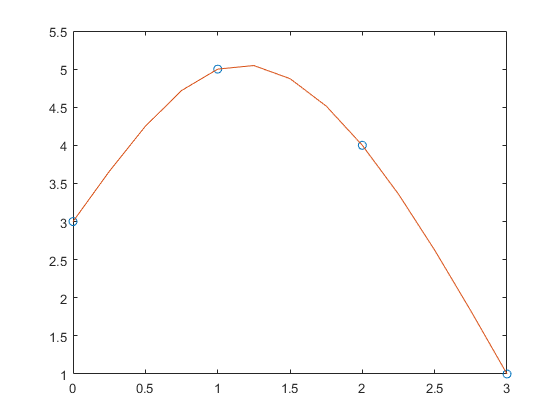
\includegraphics[scale=1]{mynd611.png}
\end{figure}
Framkvæmum nú nákvæmlega sömu skref fyrir (b) lið:

Hér keyrum við \mintinline{matlab}{splinecoeff.m} úr bók með eftirfarandi gildum
\begin{minted}{matlab}
X=[-1,0, 3, 4, 5];
Y=[3,5,1,1,1];
milta2 = splinecoeff(X,Y)
\end{minted}
Sem skilar svo:
\begin{minted}{console}
milta2 =

    2.5629         0   -0.5629
    0.8742   -1.6887    0.3176
   -0.6824    1.1698   -0.4874
    0.1950   -0.2925    0.0975
\end{minted}
höfum því eftirfarandi "spline interpolation":

\begin{align*}
S_1 &= 3+2.563(x+1)-0.563(x+1)^3\\
S_2 &= 5+0.874x-1.689x^2+0.318x^3\\
S_3 &= 1-0.682(x-3)+1.170(x-3)^2-0.487(x-3)^3\\
S_4 &= 1+0.195(x-3)-0.293(x-3)^2 + 0.098(x-3)^3
\end{align*}
fáum því næst myndina

\begin{figure}[H]
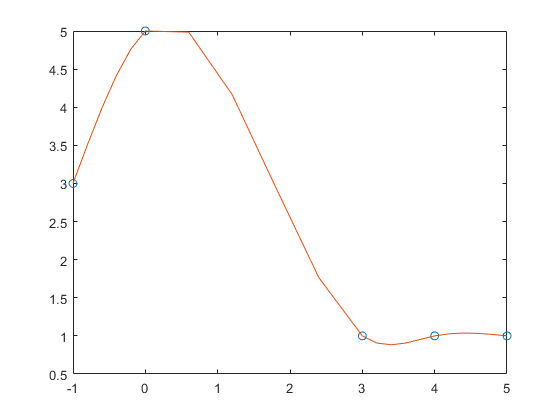
\includegraphics[scale=1]{mynd611b.png}
\end{figure}
































\end{document}
